\chapter{評価実験}
\label{chap:main_experiment}

この章では本研究で行った評価実験について述べる.
まず評価実験の概要について述べる.ついで, 本評価実験の目的を述べる.
次に, 評価実験手法およびORFにおけるデータ収集について述べた後,ユーザーの笑顔の作り方の分析を行う.
笑顔の作り方分析の後,ユーザーを自身笑顔動画データを選んだグループとそれ以外のグループにわけ,
それぞれの嗜好分析を行なった.最後に, 両方のグループから得た値から考察を行い,まとめを行なった.


\section{評価実験の概要}
本研究で作成したシステム, Delta Smile Facial Survey Analyzer(DSFSA)を使用して,
慶應義塾大学 湘南藤沢キャンパスが主催するOpen Research Forumの来場者へむけた
デモンストレーションを行いながら, ユーザーの笑顔動画データ収集および
システムによって選ばれた笑顔動画データへの順位づけを行なった.
収集したユーザー笑顔動画データをOpenFaceを用いて数値化し, 順位づけをした笑顔動画データとの間にある
嗜好傾向を分析する.

\section{評価実験の目的}
この実験の目的は, ユーザーと表情ベースにおけるユーザーの人への嗜好傾向を明らかにすることである.
本論文の第\ref{chap:introduction}章で述べた仮説は, 「表情が似ている人には好意を抱きやすい」であった.
以下では仮説検証をするとともに, 自身の表情と表情ベースにおける相手への嗜好の関係性を明らかにする.

\section{実験手法}
本論文の第\ref{chap:developing}章で述べた本システムDSFSAを使用してデータの収集を行う.
まずユーザーの中立の表情から, 笑顔になる動画データ (以下, 笑顔動画データとする)を取得する.
次に取得したフレームに対してOpenFaceを用いた処理を行い, 各FAUの値およびp\_scaleの値を取得する.
取得したp\_scaleの値を元に, ユーザー自身のデータを含む5つの笑顔動画データをシステムが選択し,
表情以外のバイアスを軽減するために顔の特徴点のみを表示した点描画をユーザーにむけて表示をする.
5つのデータに対して順位づけを行い, ユーザーの笑顔動画データのFAU, 選択された笑顔動画データのFAU
および順位づけデータをもとに分析を行い,ユーザーの笑顔の作り方と嗜好傾向を明らかにする.

\section{ORF(Open Research Forum)におけるデータ収集}
2019年11月22日金曜日と, 23日土曜日に六本木東京ミッドタウンにて慶應義塾大学湘南藤沢キャンパスが主催する
Open Research Forum(以下ORF) にて本研究のデモンストレーションおよびポスター展示をE44ブースにて行なった.
ORFにて来場者およびブースに訪れた出展者の48名に対して本システムを使用してもらった.
48個のデータの内, 破損データ7つを除く41人のデータを取得した.
さらに取得フレーム数が短い7つのデータを除く34人のデータに対して,それぞれの表情データを基にし嗜好傾向分析を行なった.

\begin{figure}[htbp]
    \begin{center}
       \fbox{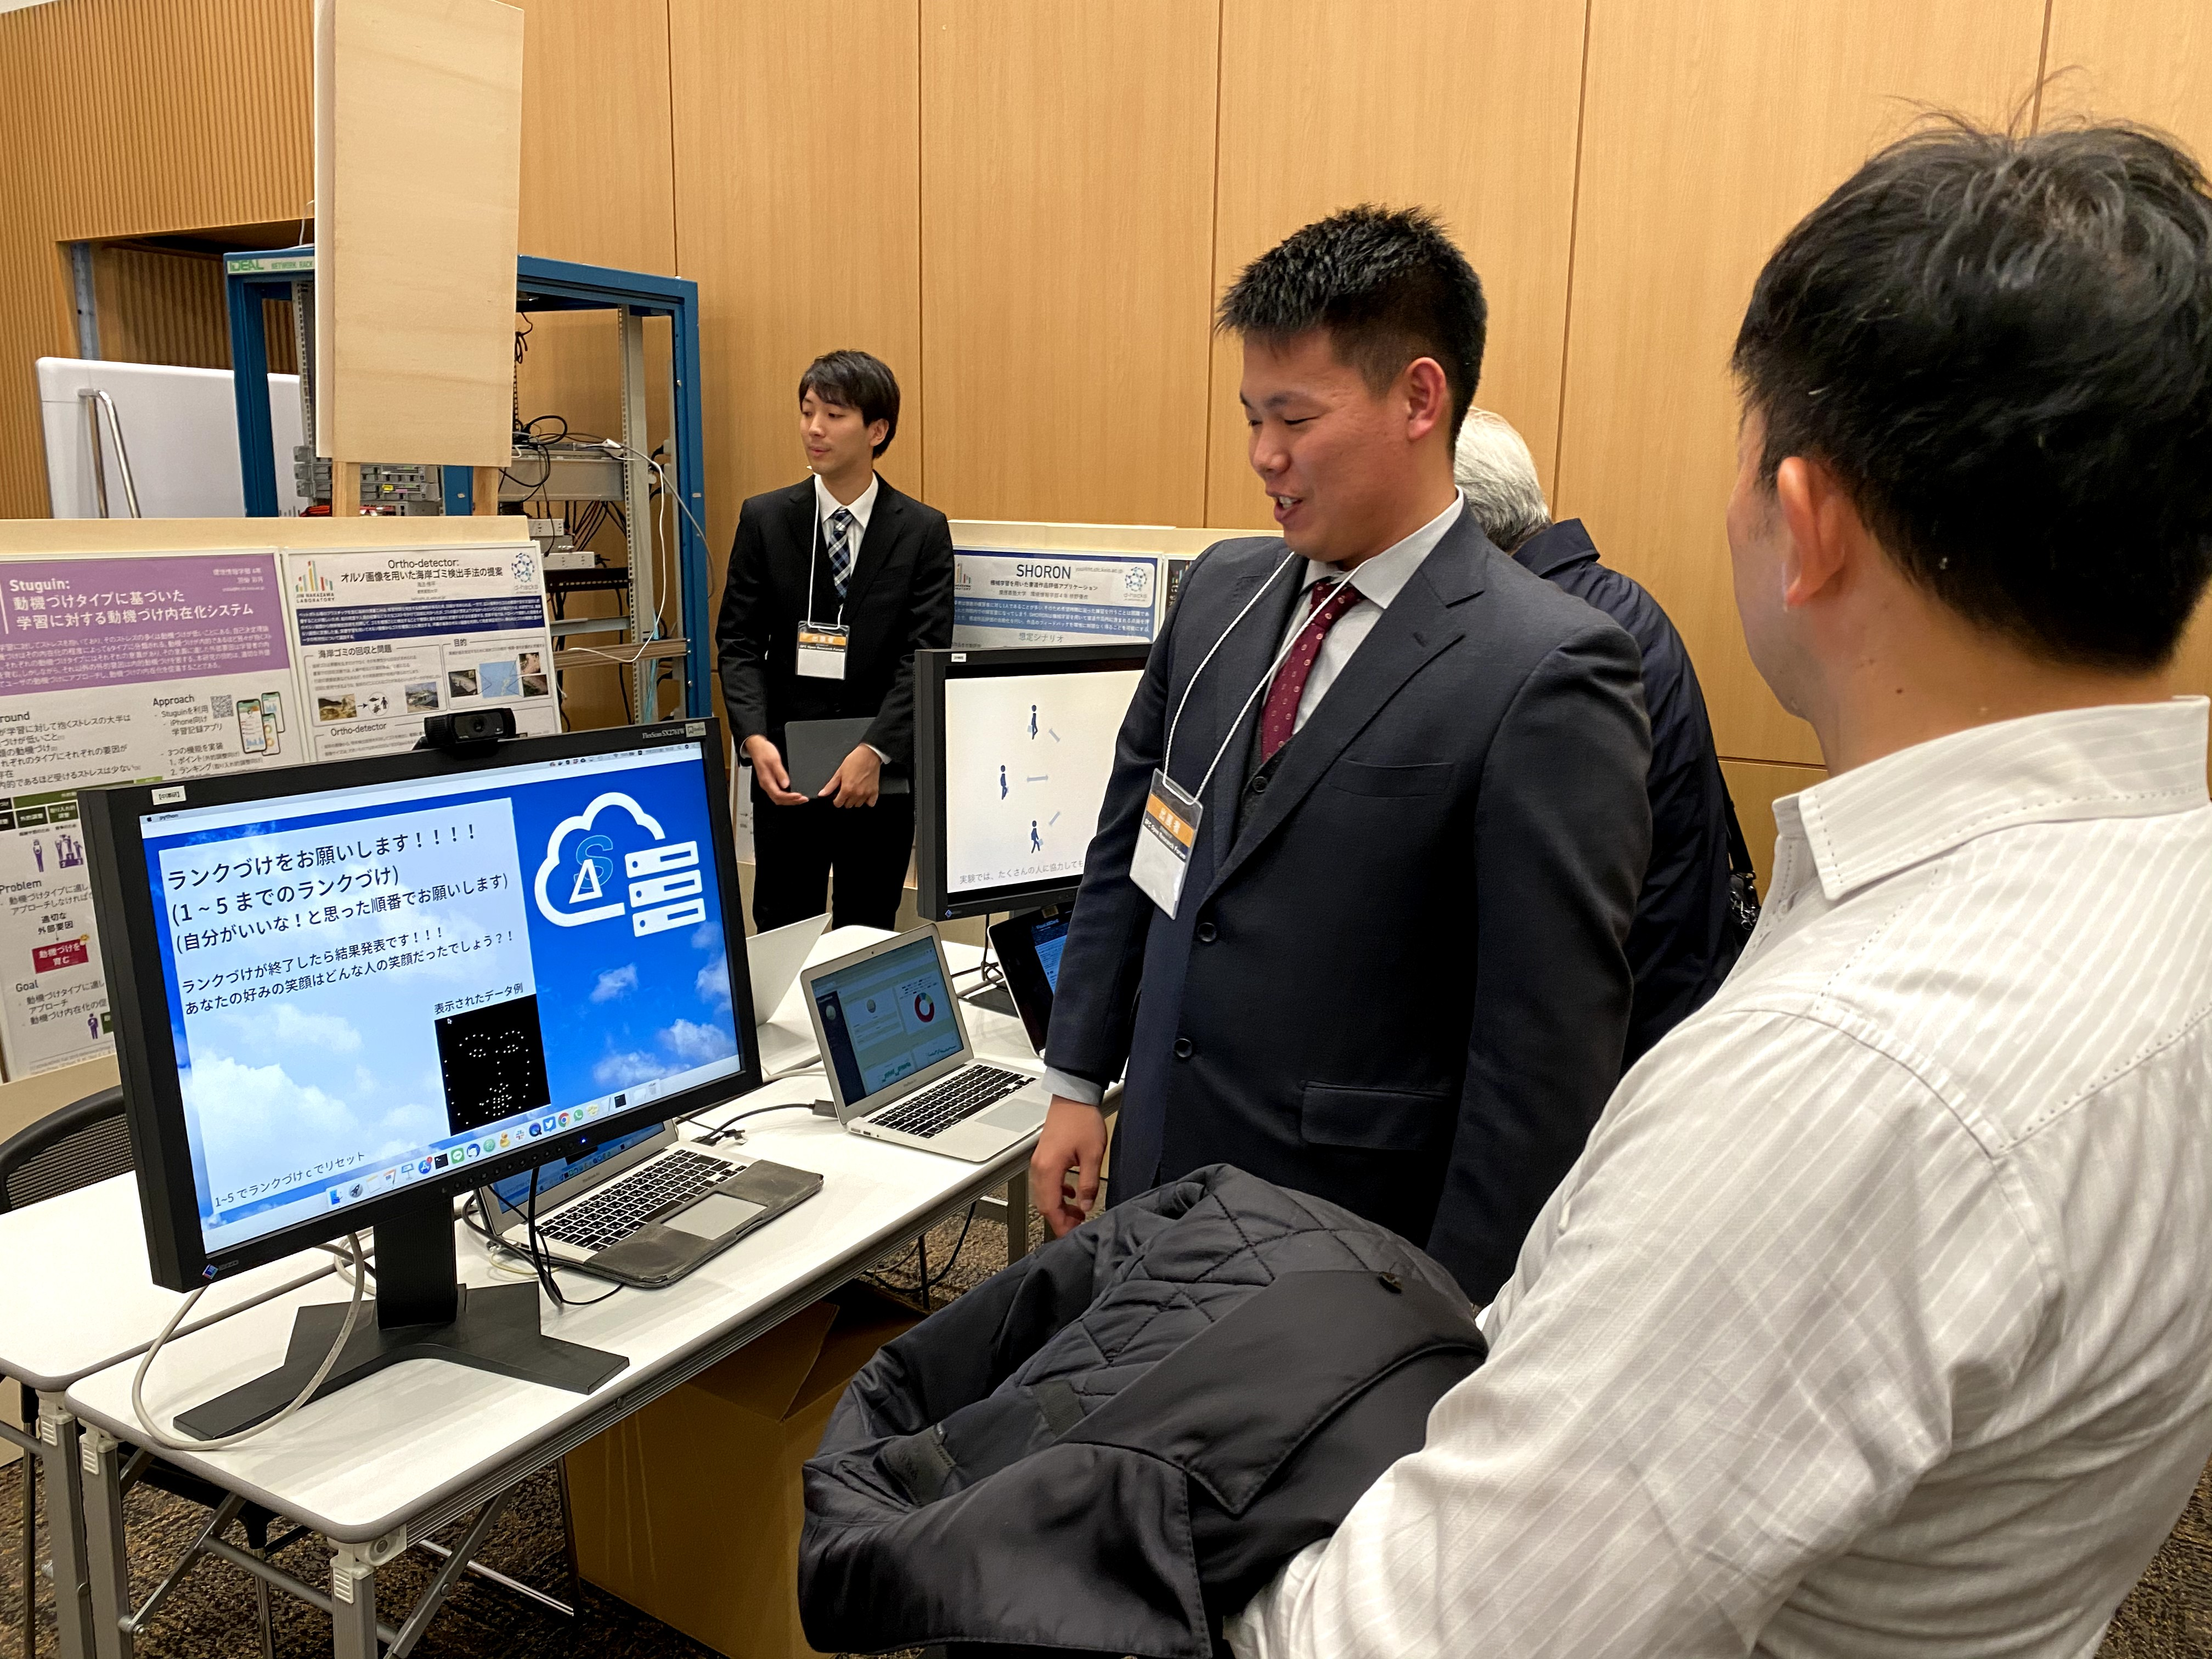
\includegraphics[width=140mm,bb=0 0 4032 3024]{20191122.jpg}}
    \end{center}
    \caption{ブースの実験の様子1}
    \label{fig:20191122}
\end{figure}

\begin{figure}[htbp]
    \begin{center}
       \fbox{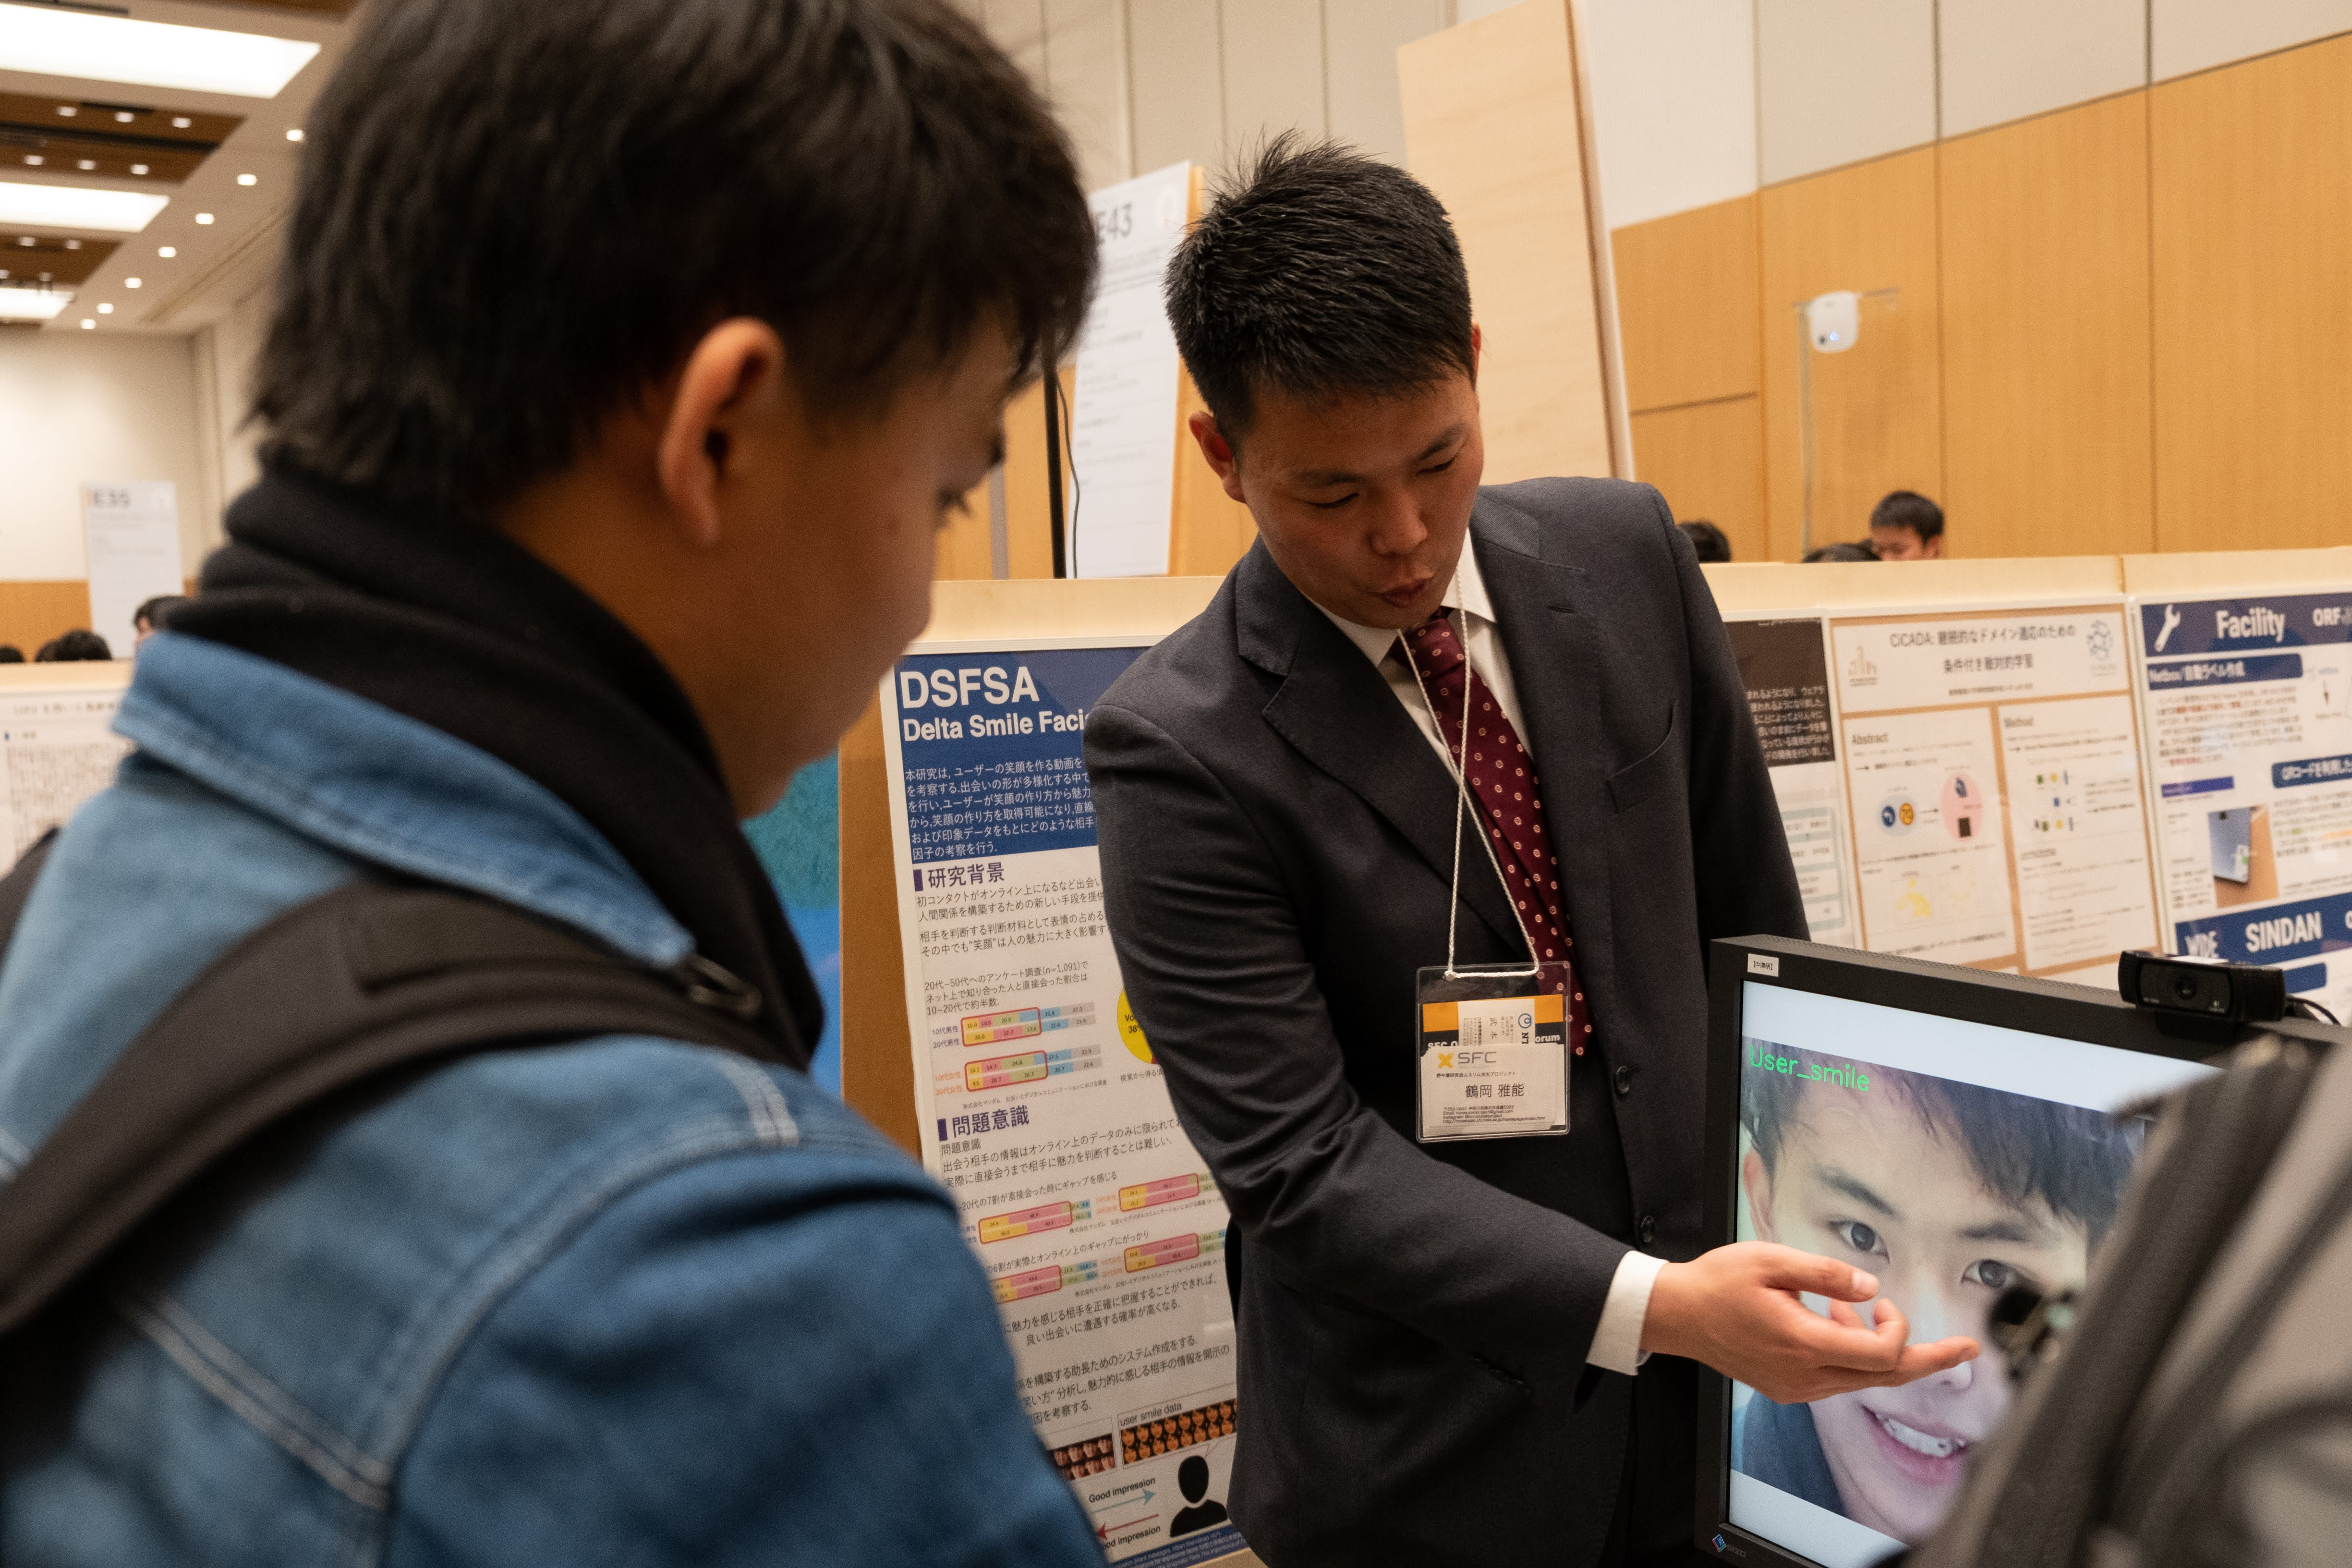
\includegraphics[width=140mm,bb=0 0 4898 3265]{20191123.jpg}}
    \end{center}
    \caption{ブースの実験の様子2}
    \label{fig:20191123}
\end{figure}

\begin{figure}[htbp]
  \begin{minipage}{0.5\hsize}
    \begin{center}
       \fbox{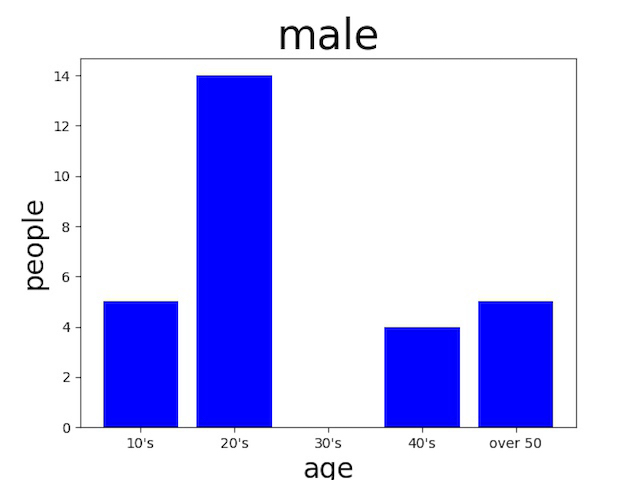
\includegraphics[width=70mm,bb=0 0 640 480]{male_graph.jpg}}
    \end{center}
    \caption{男性被験者データ(n=28)}
    \label{fig:malepeople}
  \end{minipage}
  \begin{minipage}{0.5\hsize}
    \begin{center}
       \fbox{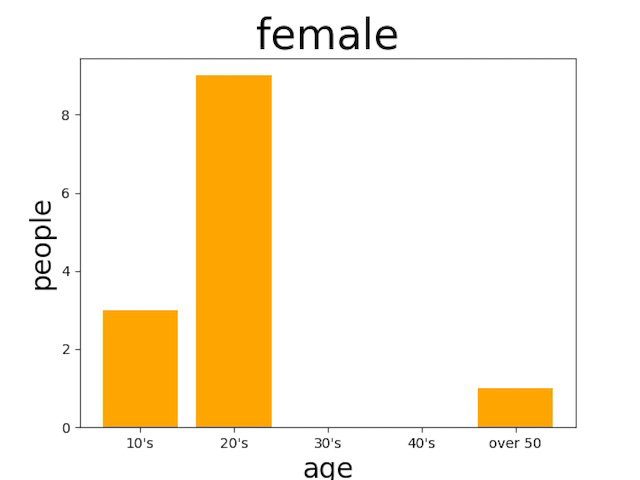
\includegraphics[width=70mm,bb=0 0 640 480]{female_graph.jpg}}
    \end{center}
    \caption{女性被験者データ(n=13)}
    \label{fig:femalepople}
  \end{minipage}
\end{figure}

\begin{table}[htb]
  \caption{被験者データ性別・年齢内訳}
  \label{tb:agegenderchart}
  \begin{center}
  \begin{tabular}{|l|r|r|r|r|r||r|} \hline
     &10代&20代&30代&40代&50代以上&合計 \\ \hline \hline
    男性&5&14&0&4&5&28 \\
    女性&3&9&0&0&1&13 \\ \hline \hline
    合計&8&23&0&4&6&41 \\ \hline
  \end{tabular}
  \end{center}
\end{table}

\section{ユーザーの笑顔の作り方の分析}
本節ではユーザーの笑顔分析をする際に使用するFAUについて述べる.
そして, ORFで取得したデータのグループ分けを行う.

\subsection{本評価実験で使用するFAUの種類}
ORFの出展にて取得したユーザーの笑顔動画データにOpenFaceを使って,Facial Action Units(以下FAU)の値の算出を行なった.
41名のユーザーデータに対して笑顔のFAU値, FAU06(眼窩部眼輪筋),07(眼瞼部眼輪筋),12(大頬骨筋),25(翼突筋+顎二腹筋)
を取得した. さらに, ユーザーが順位づけした笑顔動画データに対しても同様の処理を行い,
ユーザーのFAUの値と選んだそれぞれのユーザーのFAUの値を比較し傾向分析を行なった.

\begin{figure}[htbp]
    \begin{center}
       \fbox{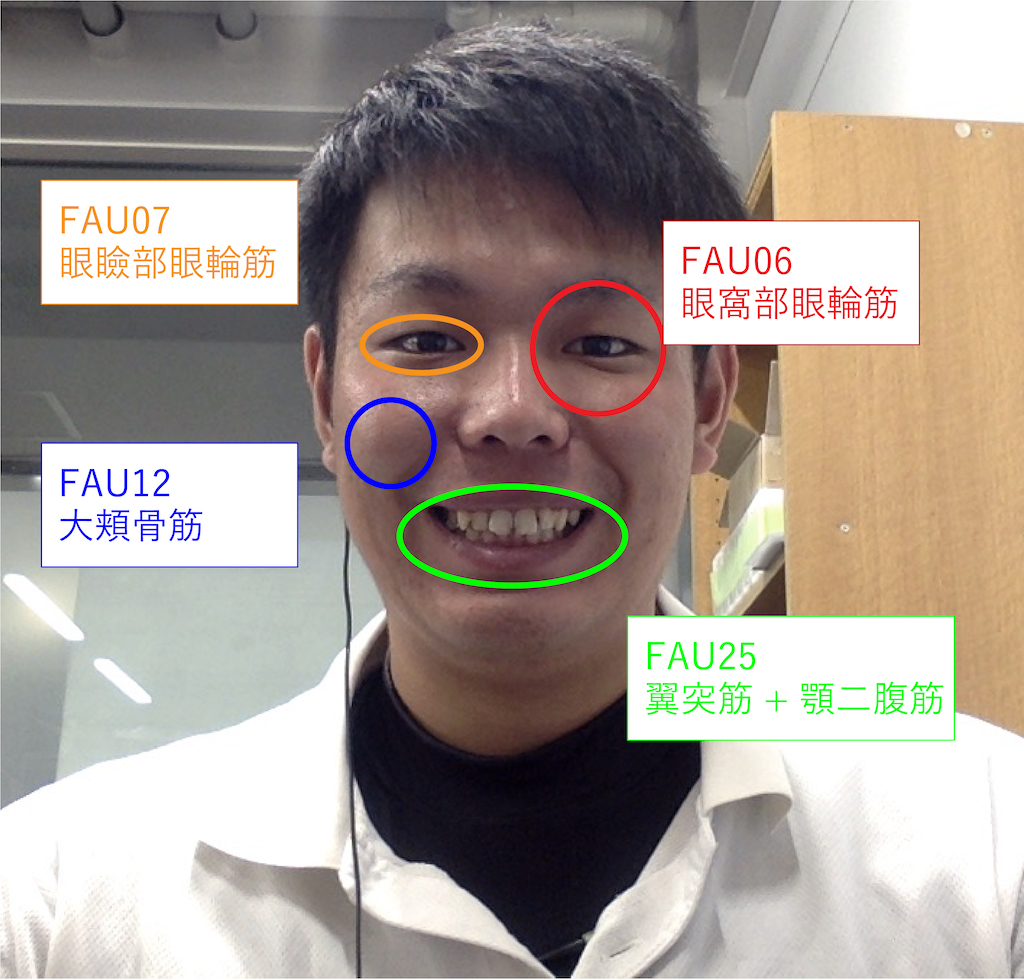
\includegraphics[width=150mm,bb=0 0 1024 980]{fau_smile.jpg}}
    \end{center}
    \caption{本研究で使用するFAUのパーツ}
    \label{fig:fau_smile}
\end{figure}

\subsection{ユーザーのグループ分け}
取得した順位づけデータをもとにユーザーを自分自身の笑顔動画データを最上位に位置づけしたユーザーと
それ以外の2種類のグループへ分類した.人数の内訳は以下のようになった.

\begin{table}[htb]
  \caption{ユーザーの笑顔動画データをもとにした分類}
  \label{tb:agegenderchart}
  \begin{center}
  \begin{tabular}{|l|r|r||r|} \hline
     &ユーザー自身&それ以外&合計 \\ \hline \hline
    男性&11&17&28 \\
    女性&4&9&13 \\ \hline \hline
    合計&14&27&41 \\ \hline
  \end{tabular}
  \end{center}
\end{table}

上記の分類の結果より, 男性は4割, 女性は3割のみが自身の笑顔動画データを選択した.
本研究の仮説である「表情が似ている人には好意を抱きやすい」は立証されなかった.
次節では, それぞれのグループごとにFAUのデータを使用して自身と似通った笑顔を持つユーザーと
それ以外のユーザーとの嗜好傾向の差分や, 共通傾向を明らかにする.
以下にはそれぞれのユーザーの4つFAUの値, それぞれ2種類のデータを表示する.
AU\_N\_c(NはFAUの番号)はFAUの値を2極値で判定をした値,AU\_N\_r(NはFAUの番号)はFAUの動きの強度を表す値である.

\begin{figure}[htbp]
    \begin{center}
       \fbox{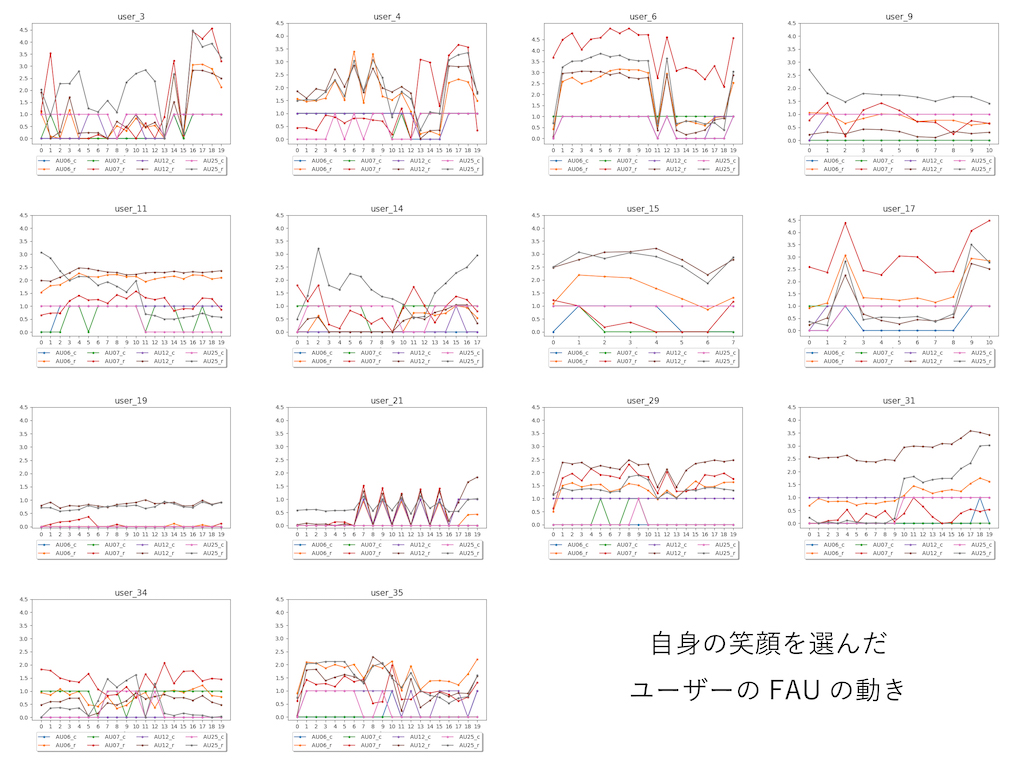
\includegraphics[width=150mm,bb=0 0 1024 768]{choice_myself_fau_for_paper.jpg}}
    \end{center}
    \caption{自身を選択したユーザーのFAUデータ}
    \label{fig:choice_myself_fau_for_paper}
\end{figure}

\begin{figure}[htbp]
    \begin{center}
       \fbox{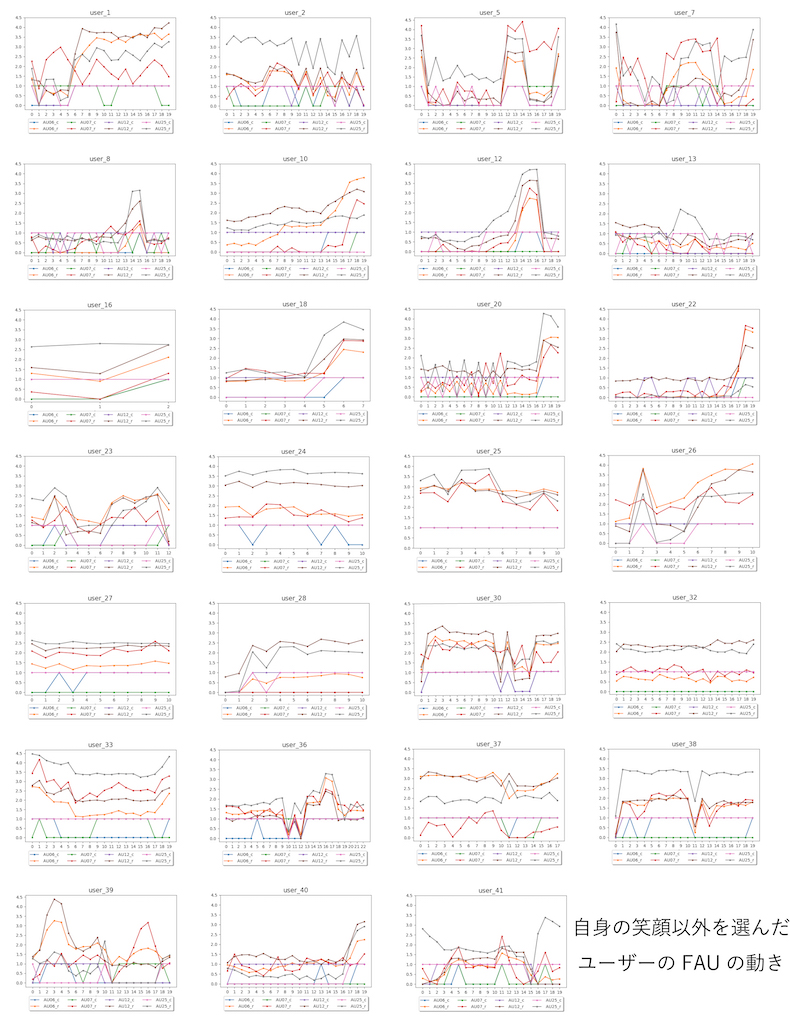
\includegraphics[width=150mm,bb=0 0 790 1024]{choose_else_for_paper.jpg}}
    \end{center}
    \caption{自身を選択しなかったユーザーのFAUデータ}
    \label{fig:choose_else_for_paper}
\end{figure}

\begin{figure}[htbp]
    \begin{center}
       \fbox{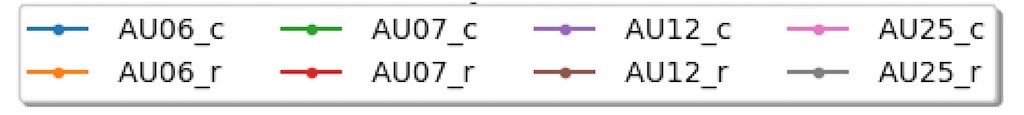
\includegraphics[width=150mm,bb=0 0 1024 115]{usage_guide_fau.jpg}}
    \end{center}
    \caption{ユーザーFAUグラフ凡例}
    \label{fig:usage_guide_fau}
\end{figure}

\section{表情をベースによる嗜好傾向分析}
本節では取得したデータから判明した傾向について述べる.
まず,性別ごとの選択傾向, 次に自身の笑顔データを選んだユーザーの選択傾向と, それ以外を選んだユーザーの選択傾向,
最後に, 共通した選択傾向について考察する.

\subsection{性別ごとの選択傾向}
本研究において, 笑顔動画データに対して順位づけをする際には, バイアスを軽減するために顔の特徴点
のみを表示し, 表情のみの判断を行なっているため性別を判断することはできない.
その上で, 男性の約64\%, 女性の約61\%無意識に同性を選んでいる弱い傾向が見られた.
また先行研究で,
U Dimbergらは, 女性のほうが笑顔になりやすく, 頬骨の筋電図に大きな刺激がでると述べており\cite{dimberg1990gender},
男性と女性では笑顔の際に筋肉の動きが少し異なることがわかっている.

またHall, Judithらは女性のほうが感情判断に優れていると述べている\cite{hall2004gender}.
しかし,L Forni-Santosらは表情の認知に関して, 男性と女性で差はないと述べている.\cite{forni2015influence}

よって, 表情ベースでの判断に性別は関係がないと考えられ, 筋肉の動きが似ている方に惹かれる弱い傾向があると言える.

性別がわからない状態では同性を選ぶ傾向にあるが, 性別を明らかにした場合は別の結果がでるかどうかを
今後, 明らかにすることができれば異性のパートナー探しをする際に, 有用なデータをとることができると考えられる.

\begin{table}[htb]
  \caption{ユーザーの笑顔動画データをもとにした分類}
  \label{tb:agegenderchart}
  \begin{center}
  \begin{tabular}{|l|r|r||r|} \hline
     &男性選択&女性選択&合計 \\ \hline \hline
    男性&18&10&28 \\
    女性&5&8&13 \\ \hline \hline
    合計&23&18&41 \\ \hline
  \end{tabular}
  \end{center}
\end{table}


\begin{figure}[htbp]
    \begin{center}
       \fbox{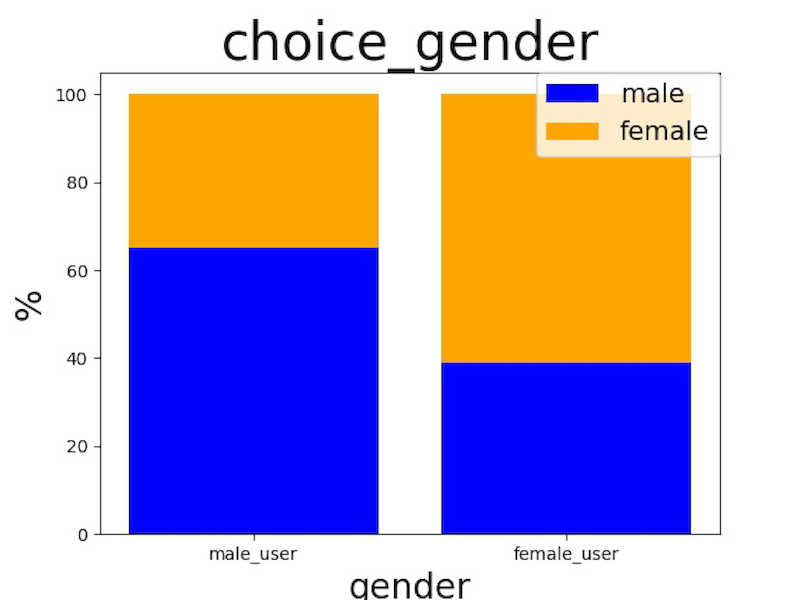
\includegraphics[width=100mm,bb=0 0 800 600]{choice_gender.jpg}}
    \end{center}
    \caption{ユーザーの性別選択}
    \label{fig:choice_gender}
\end{figure}

\subsection{自身を選択したユーザーの選択傾向}

\subsubsection{自身を選んだユーザーの特徴的データの考察}
自身を選択したユーザー全体の中で, よくみられたFAUの傾向は以下の通りである.
青い折れ線グラフは自身を選択したユーザーを示しており,一番最後のフレームにおいてFAUの値が上昇傾向にあった.
また, 直前のフレームではFAUの値が減少し, 一番最後のフレームとの差分が大きくなっていることが確認できる.
他にも, FAUの変化の値が他のフレームよりも急上昇していることより, 自分自身を選んだユーザーは笑顔の表情を作る筋肉の動きが速いこと,
表情の筋肉を緩ませてから笑顔を作る表情の動きをしていることがFAUの値の変化から読み取ることができる.

\begin{figure}[htbp]
  \begin{minipage}{0.5\hsize}
    \begin{center}
       \fbox{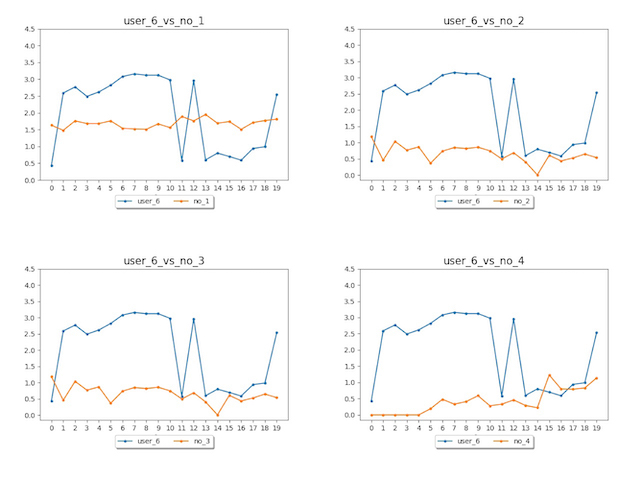
\includegraphics[width=75mm,bb=0 0 640 480]{user_fau/userfau_06.jpg}}
    \end{center}
    \caption{ユーザーFAU06}
    \label{fig:userfau_06}
  \end{minipage}
  \begin{minipage}{0.5\hsize}
    \begin{center}
       \fbox{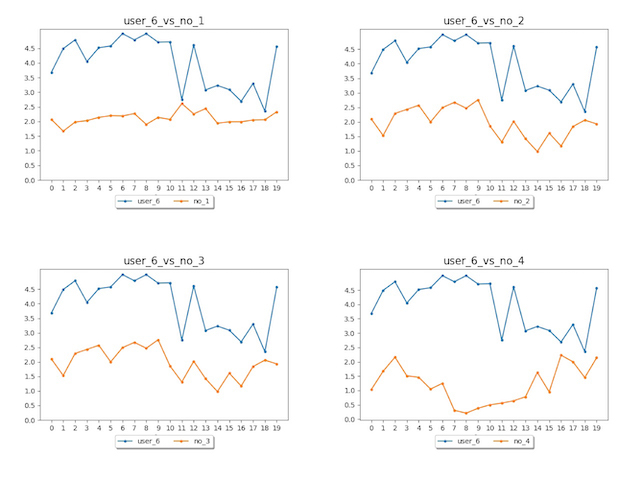
\includegraphics[width=75mm,bb=0 0 640 480]{user_fau/userfau_07.jpg}}
    \end{center}
    \caption{ユーザーFAU07}
    \label{fig:userfau_07}
  \end{minipage}
\end{figure}

\begin{figure}[htbp]
  \begin{minipage}{0.5\hsize}
    \begin{center}
       \fbox{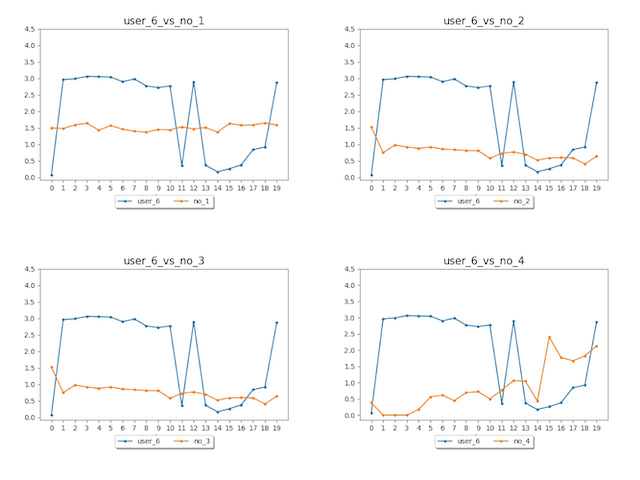
\includegraphics[width=75mm,bb=0 0 640 480]{user_fau/userfau_12.jpg}}
    \end{center}
    \caption{ユーザーFAU12}
    \label{fig:userfau_12}
  \end{minipage}
  \begin{minipage}{0.5\hsize}
    \begin{center}
       \fbox{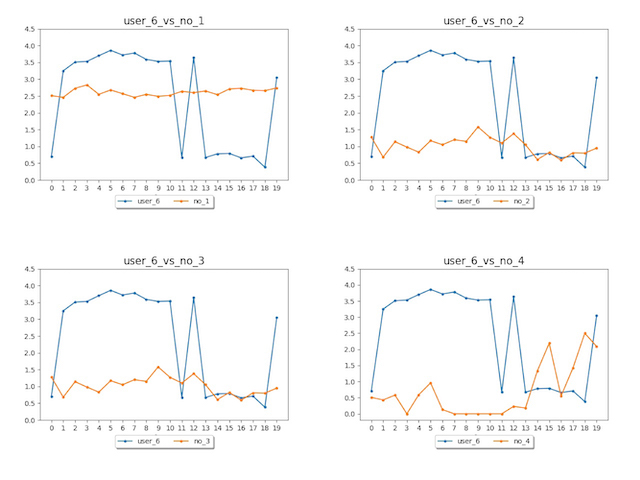
\includegraphics[width=75mm,bb=0 0 640 480]{user_fau/userfau_25.jpg}}
    \end{center}
    \caption{ユーザーFAU25}
    \label{fig:userfau_25}
  \end{minipage}
\end{figure}


\subsubsection{自身を選んだユーザーの全体考察}
自身の笑顔動画データを選んだユーザーの各FAU\_rの値を取得し, 最大値, 最小値, 範囲, 平均値, 中央値,
母分散, 標準偏差, 不偏分散を算出する.
算出した値の平均値は以下のようになった.

\begin{table}[htb]
  \caption{自身を選択したユーザーのFAUの値平均値(n=15)}
  \label{tb:choicemyself}
  \begin{center}
  \begin{tabular}{|l||r|r|r|r|r|r|r|r|} \hline
    &max	&min	&range	&mean	&median	&pvariance	&psrdeev	&variance \\ \hline \hline
  AU06	&2.032	&0.595	&1.437	&1.281	&1.239	&0.322	&0.469	&0.343 \\ \hline
  AU07	&2.288	&0.489	&1.799	&1.229	&1.093	&0.505	&0.587	&0.536 \\ \hline
  AU12	&2.274	&0.768	&1.506	&1.519	&1.506	&0.367	&0.495	&0.389 \\ \hline
  AU25	&2.724	&0.634	&2.090	&1.543	&1.548	&0.595	&0.658	&0.632 \\ \hline
  \end{tabular}
  \end{center}
\end{table}

算出した平均値より, 自身の動画データを選んだユーザーの07(眼瞼部眼輪筋),25(翼突筋+顎二腹筋)の分散および標準偏差が大きくなっている.
つまり, 自身を選んだユーザーはFAUの強度にバラつきがあり, FAUの動きが多いと考えられる.

\subsection{自身以外を選択したユーザーの選択傾向}

\subsubsection{自身以外を選んだユーザーの特徴的データの考察}
自身以外を選択したユーザー全体の中で, よくみられたFAUの傾向は以下の通りである.
青い折れ線グラフは自身を選択したユーザーを示しており,一番最後のフレームにおいてFAUの値が下降傾向にあった.
また, 直前のフレームではFAUの値が上昇し, 一番最後のフレームよりも値が大きくなっていることが確認できる.
他にも, 値が安定せず値が前のフレームと値が変化するケースが多く見られる.


\begin{figure}[htbp]
  \begin{minipage}{0.5\hsize}
    \begin{center}
       \fbox{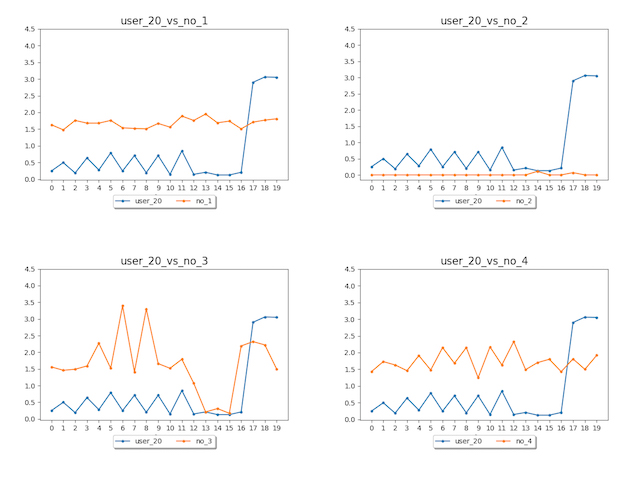
\includegraphics[width=75mm,bb=0 0 640 480]{else_fau/elsefau_06.jpg}}
    \end{center}
    \caption{ユーザーFAU06}
    \label{fig:elsefau_06}
  \end{minipage}
  \begin{minipage}{0.5\hsize}
    \begin{center}
       \fbox{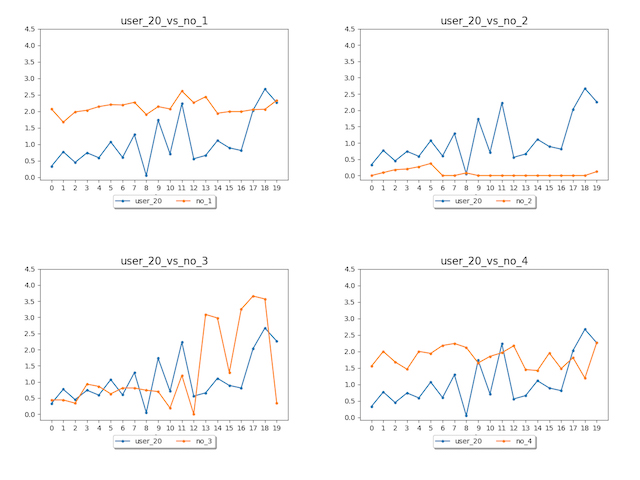
\includegraphics[width=75mm,bb=0 0 640 480]{else_fau/elsefau_07.jpg}}
    \end{center}
    \caption{ユーザーFAU07}
    \label{fig:elsefau_07}
  \end{minipage}
\end{figure}

\begin{figure}[htbp]
  \begin{minipage}{0.5\hsize}
    \begin{center}
       \fbox{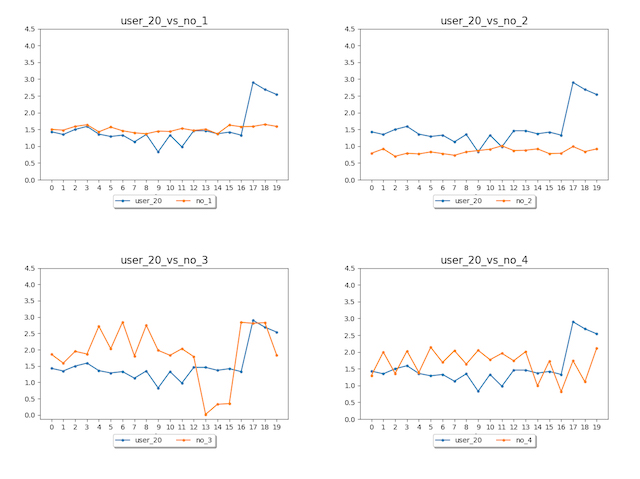
\includegraphics[width=75mm,bb=0 0 640 480]{else_fau/elsefau_12.jpg}}
    \end{center}
    \caption{ユーザーFAU12}
    \label{fig:elsefau_12}
  \end{minipage}
  \begin{minipage}{0.5\hsize}
    \begin{center}
       \fbox{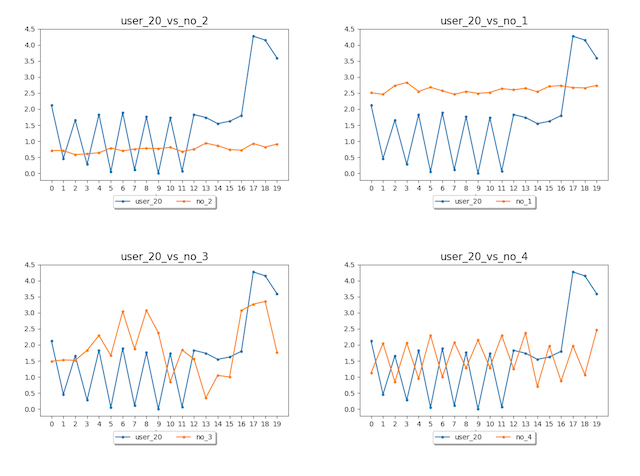
\includegraphics[width=75mm,bb=0 0 640 480]{else_fau/elsefau_25.jpg}}
    \end{center}
    \caption{ユーザーFAU25}
    \label{fig:elsefau_25}
  \end{minipage}
\end{figure}

順位づけしたFAUの観点より考察すると, このユーザーが一番上位に順位づけした笑顔動画のFAUは右下の値である.
前節でのべた傾向と同じように, 最後のフレームに置いて増加傾向にあるユーザーを選んでいる傾向がみられる.

\subsubsection{自身以外を選んだユーザーの全体考察}
自身の笑顔動画データを選んだユーザーと, ユーザーが選んだ笑顔動画データの各FAU\_rの値を取得し, 最大値, 最小値, 範囲, 平均値, 中央値,
母分散, 標準偏差, 不偏分散を算出する.
算出した値の平均値は以下のようになった.

\begin{table}[htb]
  \caption{自身以外を選択したユーザーのFAUの値平均値(n=21)}
  \label{tb:choiceelse}
  \begin{center}
  \begin{tabular}{|l||r|r|r|r|r|r|r|r|} \hline
    &max	&min	&range	&mean	&median	&pvariance	&psrdeev	&variance \\ \hline \hline
  AU06	&2.364	&0.368	&1.996	&1.147	&1.066	&0.489	&0.621	&0.516 \\ \hline
  AU07	&2.510	&0.311	&2.199	&1.204	&1.092	&0.537	&0.625	&0.566 \\ \hline
  AU12	&2.860	&0.690	&2.170	&1.608	&1.562	&0.540	&0.659	&0.570 \\ \hline
  AU25	&3.030	&0.764	&2.266	&1.810	&1.780	&0.557	&0.660	&0.588 \\ \hline
  \end{tabular}
  \end{center}
\end{table}

\begin{table}[htb]
  \caption{自身以外を選択したユーザーが選んだ笑顔動画データのFAUの値平均値(n=21)}
  \label{tb:elsechoice}
  \begin{center}
  \begin{tabular}{|l||r|r|r|r|r|r|r|r|} \hline
    &max	&min	&range	&mean	&median	&pvariance	&psrdeev	&variance \\ \hline \hline
  AU06	&1.889	&0.754	&1.135	&1.242	&1.194	&0.193	&0.338	&0.204 \\ \hline
  AU07	&2.535	&0.877	&1.658	&1.692	&1.680	&0.430	&0.481	&0.454 \\ \hline
  AU12	&2.121	&0.778	&1.343	&1.352	&1.278	&0.295	&0.407	&0.312 \\ \hline
  AU25	&2.907	&1.370	&1.538	&2.182	&2.251	&0.365	&0.444	&0.385 \\ \hline
  \end{tabular}
  \end{center}
\end{table}

算出した平均値より, 選ばれた笑顔動画データはFAU06(眼窩部眼輪筋),12(大頬骨筋)の分散, 標準偏差の値が自身のFAUの値に比べ小さくなっている.
さらに値の範囲(最大値-最小値)の値も, ユーザーのデータよりも小さい値を示している.
これより, 自身以外のデータを選んだユーザーは表情の変化が小さいデータ,また安定した表情の動きをした笑顔を好む傾向があることがわかった.

\subsection{共通した嗜好傾向}
ユーザーのFAU値において, 両グループともに順位づけが一番高いデータは最後のフレームとその前のフレームとのFAUの値の差分が大きく,
かつ上昇傾向であるデータであることが確認できる.
つまり, 一度顔の筋肉を弛緩させてから笑顔になる笑顔動画データが選択されることが本実験でわかった.
各グループの4つのFAU値の平均値の差分は以下のようになった.
表\ref{tb:mean_differences}より, 自身以外を選択したユーザーのほうがFAUの値は平均して高く, 値が分散していることがわかる.

\begin{table}[htb]
  \caption{FAU平均値差分[(自分自身選択ユーザー)-(自身以外選択ユーザー)]}
  \label{tb:mean_differences}
  \begin{center}
  \begin{tabular}{|l||r|r|r|r|r|r|r|r|} \hline
    &max	&min	&range	&mean	&median	&pvariance	&psrdeev	&variance \\ \hline \hline
  AU06	&-0.332 	&0.227 	&-0.558 	&0.134 	&0.172 	&-0.167 	&-0.152 	&-0.173   \\ \hline
  AU07	&-0.222 	&0.177 	&-0.399 	&0.025 	&0.001 	&-0.032 	&-0.038 	&-0.030   \\ \hline
  AU12	&-0.586 	&0.078 	&-0.664 	&-0.088 	&-0.056 	&-0.173 	&-0.164 	&-0.181   \\ \hline
  AU25	&-0.306 	&-0.130 	&-0.176 	&-0.268 	&-0.233 	&0.038 	&-0.002 	&0.044   \\ \hline
  \end{tabular}
  \end{center}
\end{table}


\section{自身の表情の作り方と好感をもつ笑顔との関係性}
上記の分析結果より, 人は一度顔の筋肉を弛緩してから笑顔になるユーザーに対して嗜好傾向が
ある可能性を本研究において示す.
表\ref{tb:prefer_fau}に順位づけデータが1番上の各FAU\_r最大値, 最小値, 範囲, 平均値, 中央値,
母分散, 標準偏差, 不偏分散の平均値を算出した.
嗜好傾向にある笑顔は, 笑顔の基準FAU06(眼窩部眼輪筋),12(大頬骨筋)の分散値が小さく,
最大値および最小値が表の値に収束するような値が望ましいと言える.

\begin{table}[htb]
  \caption{嗜好傾向にあった動画データのFAU平均値(n=36)}
  \label{tb:prefer_fau}
  \begin{center}
  \begin{tabular}{|l||r|r|r|r|r|r|r|r|} \hline
    &max	&min	&range	&mean	&median	&pvariance	&psrdeev	&variance \\ \hline \hline
  AU06	&1.948	&0.688	&1.261	&1.258	&1.213	&0.247	&0.393	&0.262   \\ \hline
  AU07	&2.432	&0.715	&1.717	&1.499	&1.436	&0.461	&0.525	&0.488   \\ \hline
  AU12	&2.185	&0.774	&1.411	&1.422	&1.373	&0.325	&0.444	&0.344   \\ \hline
  AU25	&2.831	&1.063	&1.768	&1.916	&1.958	&0.461	&0.533	&0.488   \\ \hline
  \end{tabular}
  \end{center}
\end{table}

\section{まとめ}
本節では評価実験についてまとめ, 結果と分析結果からわかる可能性について述べた.
次章では, 本研究における結論および今後の展望について述べる.
